%%%%%%%%%%%%%%%%%%%%%%%%%%%%%%%%%%%%%%%%%%
%%%%%%%%%%%%%                 %%%%%%%%%%%%
%%%%%%%%%%%%%    EXERCISE 1   %%%%%%%%%%%%
%%%%%%%%%%%%%                 %%%%%%%%%%%%
%%%%%%%%%%%%%%%%%%%%%%%%%%%%%%%%%%%%%%%%%%
\begin{exercise}[]{
    Please explain the differences between structural hazards, data hazards, control hazards.
    }
  \begin{solution}
  \par{~}
  \begin{enumerate}
      \item Structural hazards arise from resource conflicts when the hardware cannot support all possible combinations of instructions simultaneously in overlapped execution. For example, a register can't be read and written at the same time.
      \item Data hazards arise when an instruction depends on the results of a previous instruction in a way that is exposed by the overlapping of instructions in the pipeline. For example, when pipelining, read after write hazards can happen, when the data is not actually written back into the register but is requested by the next read instruction.
      \item Control hazards arise from the pipelining of branches and other instructions that change the PC. For example, when a branching instruction modifies the PC, the following instructions after the branching instruction may have been loaded into the pipeline execution, which need to be abandoned.
  \end{enumerate}
  \end{solution}
  \label{ex1}
\end{exercise}


%%%%%%%%%%%%%%%%%%%%%%%%%%%%%%%%%%%%%%%%%%
%%%%%%%%%%%%%                 %%%%%%%%%%%%
%%%%%%%%%%%%%    EXERCISE 2   %%%%%%%%%%%%
%%%%%%%%%%%%%                 %%%%%%%%%%%%
%%%%%%%%%%%%%%%%%%%%%%%%%%%%%%%%%%%%%%%%%%
\begin{exercise}[]{Identify all of the data dependences in the following code. Which dependences are data hazards that will be resolved via forwarding?}
    \begin{verbatim}
        ADD r2,r5,r4
        ADD r4,r2,r5
        SW r5,100(r2)
        ADD r3,r2,r4 
    \end{verbatim}
  \begin{solution}
  \par{~}
  Data Dependence:
  \begin{enumerate}
      \item \texttt{ADD r2,r5,r4} and \texttt{ADD r4,r2,r5} on \texttt{r2}
      \item \texttt{ADD r2,r5,r4} and \texttt{SW r5,100(r2)} on \texttt{r2}
      \item \texttt{ADD r2,r5,r4} and \texttt{ADD r3,r2,r4} on \texttt{r2}
      \item \texttt{ADD r4,r2,r5} and \texttt{ADD r3,r2,r4} on \texttt{r4}
  \end{enumerate}
  (1), (2) and (4) can be solved by forwarding ALU results. (3) will not cause data hazards in MIPS pipeline.
  \end{solution}
  \label{ex2}
\end{exercise}

%%%%%%%%%%%%%%%%%%%%%%%%%%%%%%%%%%%%%%%%%%
%%%%%%%%%%%%%                 %%%%%%%%%%%%
%%%%%%%%%%%%%    EXERCISE 3   %%%%%%%%%%%%
%%%%%%%%%%%%%                 %%%%%%%%%%%%
%%%%%%%%%%%%%%%%%%%%%%%%%%%%%%%%%%%%%%%%%%
\begin{exercise}[]{
    \item Please write a program in OpenMP, to compute the sum of a vector. Requirements are as follows.
    \begin{itemize}
        \item Serial implement function of vector sum and parallel function of vector sum should be included.
        \item Use the time of serial implement function as baseline, and test the time acceleration ratio of arrays in different length under parallel function. 
        \item Code, result should be shown in this assignment.
    \end{itemize}}
  \begin{solution}
  \par{~}

  The implementation C++ code is shown below. A running example can be found in Figure \ref{fig:ex3}

  \begin{table}[p]
    \begin{center}
      \begin{tabular}{llllllll}
      \hline
      \multicolumn{1}{c}{\textbf{Array Size}} & \multicolumn{1}{c}{10} & \multicolumn{1}{c}{100} & \multicolumn{1}{c}{1000} & \multicolumn{1}{c}{\textbf{$10^4$}} & \multicolumn{1}{c}{\textbf{$10^5$}} & \multicolumn{1}{c}{\textbf{$10^6$}} & \multicolumn{1}{c}{\textbf{$10^7$}} \\ \hline
SpeedUp Ratio                           & 0.00086                         & 0.00359                          & 0.02345                           & 0.13191                             & 1.19131                             & 1.75058                             & 3.99408                             \\ \hline

      \end{tabular}
    \end{center}
    \caption{SpeedUp Ratio VS Array Size (4 threads)}
  \end{table}

  \begin{figure}[p]
    \begin{center}
        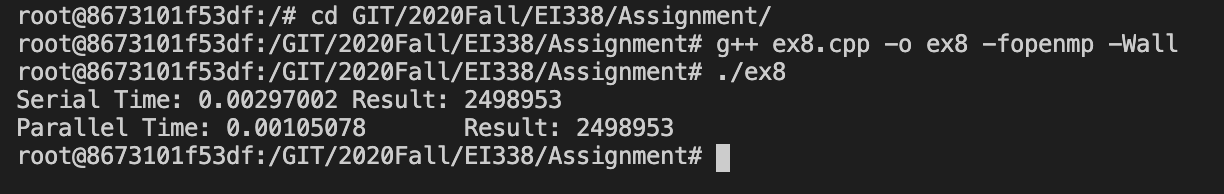
\includegraphics[width=0.5\linewidth]{ex8.png}
        \caption{A running example of the openMP program}
        \label{fig:ex3}
    \end{center}
  \end{figure}



  \end{solution}
  \label{ex3}
\end{exercise}


\begin{verbatim}
  #include<omp.h>
  #include<iostream>
  #include<fstream>

  using namespace std; 

  int* generate_array(int len, int randl, int randr){
      int* gen = new int [len];
      for (int i=0; i<len; ++i){
          gen[i] = rand() % (randr - randl + 1) + randl;
      }
      return gen;
  }

  int serial_sum(int* arr, int len){
      int sum = 0;
      for (int i=0; i<len; ++i){
          sum += arr[i];
      }
      return sum;
  }

  int parallel_sum(int* arr, int len){
      int sum = 0;
      # pragma omp parallel for num_threads(4) reduction(+:sum)
      for (int i=0; i<len; ++i){
          sum += arr[i];
      }
      return sum;
  }

  int main(int argc, char* argv[]){
      int m = 1000000, l = 0, r = 5;
      // generate a random array with 1000 elements ranging from 0 to 4;
      int* arr = generate_array(m,l,r);

      double t1,t2,t3;
      t1 = omp_get_wtime();
      int sum_res1 = serial_sum(arr, m);
      t2 = omp_get_wtime();
      int sum_res2 = parallel_sum(arr, m);
      t3 = omp_get_wtime();
      cout << "Serial Time: " << t2 - t1 << "\tResult: " << sum_res1 << endl;
      cout << "Parallel Time: " << t3 - t2 << "\tResult: " << sum_res2 << endl;
      delete [] arr;
      return 0;
  }
\end{verbatim}